\documentclass[11pt]{article}
\usepackage{graphicx}
\usepackage{float}
\usepackage{amsmath}
\usepackage{amsfonts}
\usepackage[brazilian]{babel}
\usepackage[utf8]{inputenc}
\usepackage[T1]{fontenc}

\begin{document}

\title{Matemática Elementar: Introdução a Funções}
\author{Erik Perillo}
\date{}
\maketitle
\begin{abstract}
Nesta etapa, vamos falar de um dos conceitos mais importantes para o cálculo.
\end{abstract}

\newpage

\tableofcontents

\newpage

\section{Introdução}
\paragraph{}
No dia a dia, precisamos o tempo todo relacionar um certo número com outro.
Por exemplo: se queremos saber o quanto vamos gastar para comprar um certo
número de salgadinhos de 2 reais cada, podemos pensar que o preço que vamos 
pagar é duas vezes o número de salgadinhos! Se chamarmos o número de 
salgadinhos de n e o preço de p, podemos escrever matematicamente:
$$p = 2*n$$
Ou até mesmo:
$$p(n) = 2*n$$
Ou seja, $p$ é um número que depende de $n$. Assim, escrevemos $p(n)$.
\paragraph{} 
No exemplo acima, notamos que $p$ é um valor que depende de $n$. Não se pode
determinar $p$ sem saber $n$ primeiro. Assim, dizemos que $p$ é uma variável
\textbf{dependente} e que $n$ é uma variável \textbf{independente}. Uma 
relação como essas é o que chamamos de \emph{função}.
\paragraph{}
Pensando que o número dependente da função só é sabido quando temos o termo
independente, podemos pensar em uma pequena máquina, onde na entrada colocamos 
nossa variável independente e na saída colocamos o resultado da função. A
máquina, então, seria a função nessa analogia.

\begin{figure}[H]
  		\centering
    	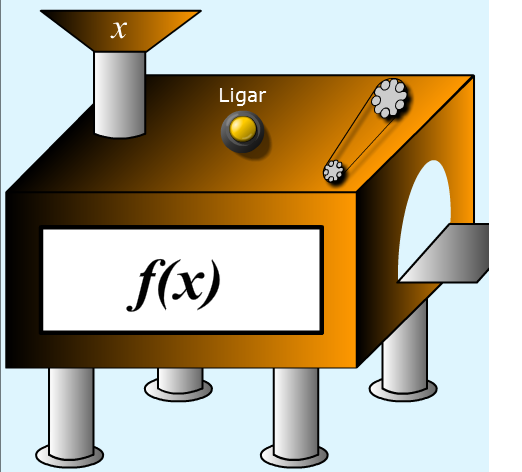
\includegraphics[width=0.5\textwidth]{imgs/funcao.png}
		\caption[9pt]{Uma função como uma máquina}
\end{figure}

\section{Um exemplo de função}
\paragraph{}
Suponha que o dono de uma lojinha de $1,99$ quer calcular quanto ele vai lucrar
com a venda de bichinhos de pelúcia. Ele comprou $15$ bichinhos, a $3,50$ cada
um, e pretende vendê-los a $6$ reais cada um. Como podemos calcular isso?
\paragraph{}
Bom, primeiro vamos deixar claro que lucro é quanto você ganha na venda de 
alguma coisa tirando quanto você gastou nela. Assim, se eu comprar uma bala
por um real e vendê-la a $1,50$, eu tive cinquenta centavos ($1,50 - 1$) de 
lucro. No caso do nosso vendedor, ele já gastou dinheiro com seus $15$
ursinhos. O total investido foi $15*3,50 = 52,50$. 
\paragraph{}
O que falta agora? Precisamos de um jeito de calcular quanto dinheiro ele vai 
ganhar com a venda dos ursinhos a $6$ reais cada um. Mas perceba: 
isso \emph{depende} de quantos ursinhos ele vai vender! 
Notamos então que podemos pensar que 
\textbf{o lucro do vendedor é uma função de quantos ursinhos ele vende}! 
Quanto ele ganha em valor bruto de acordo com o número de ursinhos? Fácil.
Chamando o número de ursinhos vendidos de $x$, percebemos que quanto ele ganha
em bruto é $6x$ (já que o preço de cada ursinho é $6$ reais). Isso é só o 
bruto. Lembrando o que o lucro é, precisamos tirar desse valor o dinheiro que 
ele investiu ($52.5$ reais). Juntando tudo e chamando o lucro de $y$, temos:
$$y(x) = 6x - 52.5$$

\subsection{Ilustrando uma função}
\paragraph{}
Vamos continuar no caso da lojinha acima e pensar em alguns casos de lucro.
Vamos pensar no caso em que ele vende $0$, $5$, $10$, e $15$ ursinhos e ver
o lucro em cada um desses casos:
\newline
\newline
\begin{tabular}{|l | r|}
	\hline
	número de ursos vendidos & lucro \\
	\hline
	$0$ & $-52.5$ \\	
	$5$ & $-22.5$ \\	
	$10$ & $7.5$ \\	
	$15$ & $37.5$ \\	
	\hline
\end{tabular}
\paragraph{}
Quando o lucro é negativo, quer dizer que ele perdeu dinheiro. 
Como podemos ilustrar isso como um gráfico no \emph{plano cartesiano}? 
\subsubsection{Plano cartesiano}
\paragraph{}
Vamos parar nosso exemplo por um minuto para falar sobre o que é um plano
cartesiano. Um plano cartesiano nada mais é que um espaço onde você pode 
desenhar suas funções para ter uma ideia de como elas se comportam:
\begin{figure}[H]
  		\centering
    	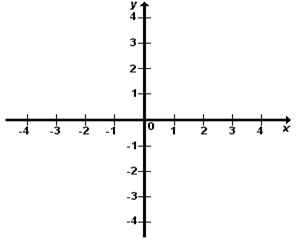
\includegraphics[width=0.5\textwidth]{imgs/plano_cartesiano.jpg}
		\caption[9pt]{Um plano cartesiano}
\end{figure}
Vamos notar algumas coisas: Olha pro eixo horizontal. Não tem um x desenhado 
lá? É nesse eixo que, geralmente, representamos a variável independente do 
nosso gráfico. O chamamos de eixo da \emph{abcissa}. No eixo vertical, com
um y desenhado, representamos os valores da função de acordo com os valores
de entrada em x.
\paragraph{}
Voltando ao nosso exemplo, vamos desenhar os valores da tabela em um plano
cartesiano:
\begin{figure}[H]
  		\centering
    	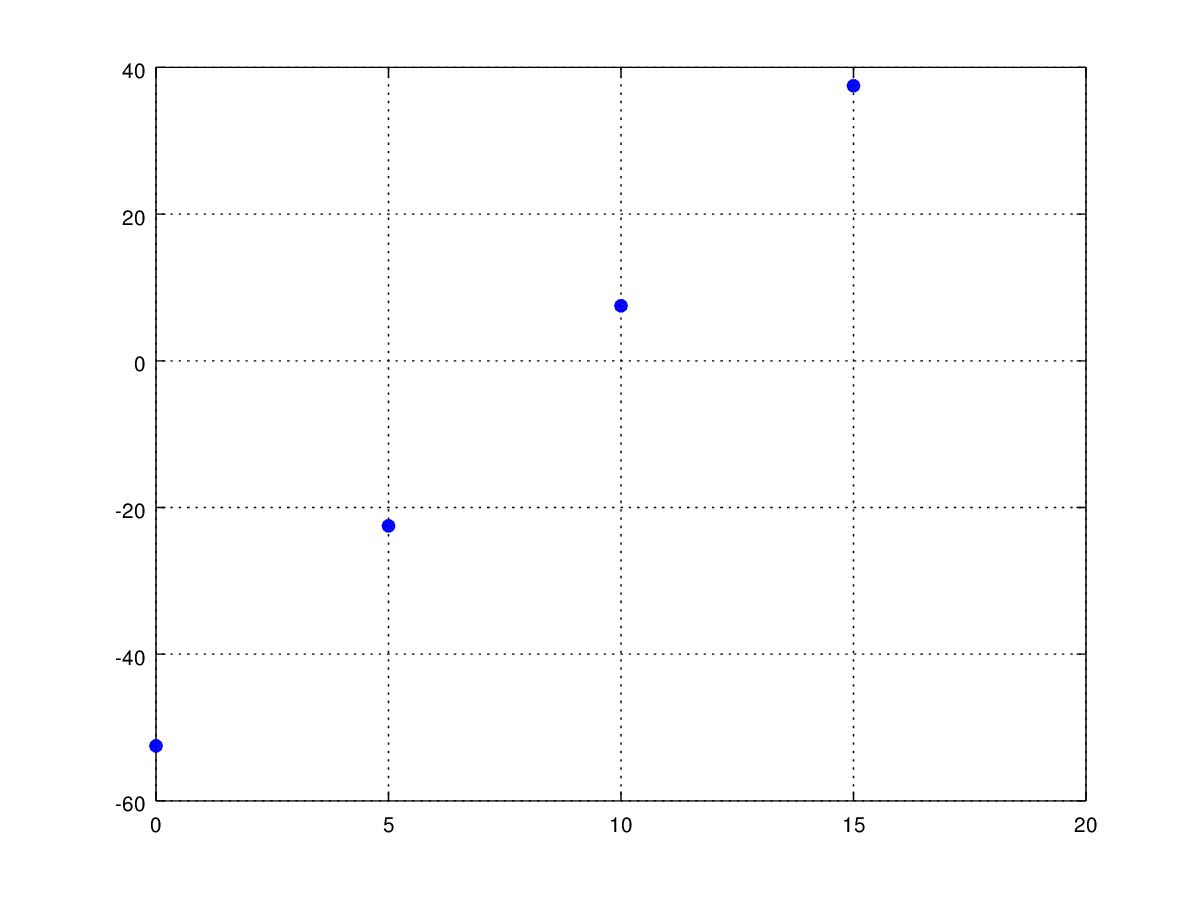
\includegraphics[width=0.5\textwidth]{imgs/grafico.png}
		\caption[9pt]{Pontos da função lucro}
\end{figure}
Note que no eixo $x$, colocamos o valor de ursinhos vendidos (variável 
independente) e, a cada um desses valor, há o valor de lucro correspondente
no eixo y.
\paragraph{}
Podemos notar que há uma linha que liga os pontos. Se plotarmos toda a linha,
teremos o seguinte:
\begin{figure}[H]
  		\centering
    	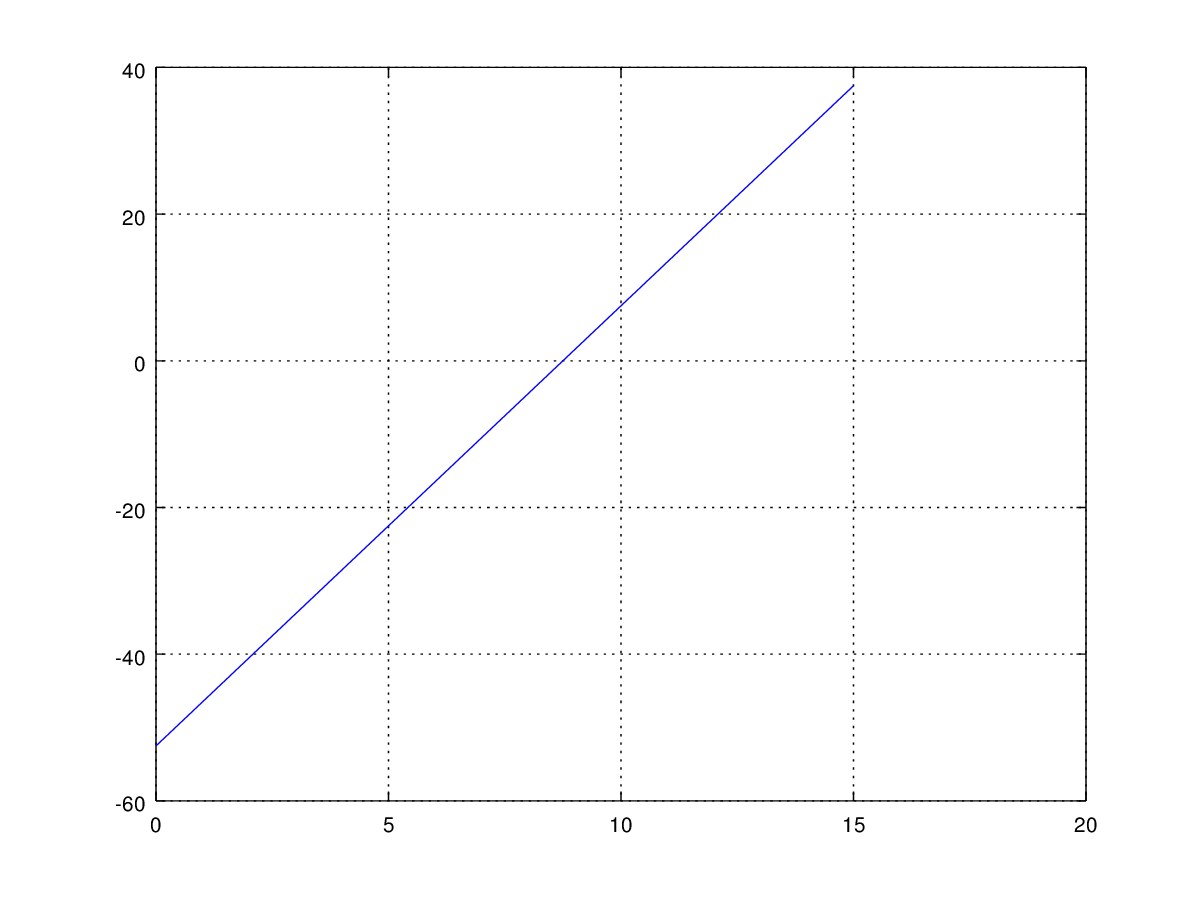
\includegraphics[width=0.5\textwidth]{imgs/linha.png}
		\caption[9pt]{Linha da função lucro}
\end{figure}
Notamos que essa é uma função \emph{linear}. E pronto, agora já temos uma
ideia melhor do que é uma função!

\section{Características de uma função}
\paragraph{}
Vamos entender nesta seção algumas coisas que cada função tem.

\subsection{O que é preciso para se ter uma função?}
\paragraph{}
Há apenas uma regra para funções: \textbf{Uma função deve ter uma, e apenas 
uma saída para cada entrada.} Isso quer dizer que não podemos ter uma função
\textit{f(x)} tal que, por exemplo, $f(2) = 5$ e $f(2) = 7$. Para o valor 
$2$, só pode ter apenas um valor correspondente, ou 5 ou 7, mas nunca os 
dois. Note que isso não impede de haver o mesmo valor de saída para duas
entradas diferentes: $f(3) = 4$ e $f(5) = 4$ é permitido, por exemplo.

\subsection{Domínio e Contradomínio}
\paragraph{}
Uma função precisa ter bem definido qual o \emph{tipo de entrada} e o 
\emph{tipo de saída} que ela vai ter, isto é: a qual \emph{conjunto} 
pertencem os valores aceitáveis de entrada e a qual \emph{conjunto} pertencem
os valores aceitáveis de saída. Ao conjunto dos valores de entrada, damos
o nome de \textbf{domínio}, e aos de saída, \textbf{contradomínio}.
\paragraph{}
No exemplo do vendedor, notamos que os valores de entrada só podem ser 
\emph{naturais}. Não faz sentido vender meio ursinho ou ainda $-1$ ursinho.
Na saída, temos números quebrados, então podemos falar que o lucro pertence
aos \emph{reais}. Assim, seu domínio é $\mathbb{N}$ e seu contradomínio 
é $\mathbb{R}$. Podemos então descrever a função de lucro $f(x)$ como:
$$f(x): \mathbb{N} \rightarrow \mathbb{R}$$

\subsection{Raízes de uma função}
\paragraph{}
No exemplo do vendedor de ursinhos, seria interessante saber qual o número 
mínimo de ursinhos que deve-se vender para não sair no prejuízo, né? Como
poderíamos fazer isso?
\paragraph{}
Vamos notar primeiramente que, para se ter algum lucro, eu não posso ter
prejuízo nenhum. Para não se ter prejuízo, o valor da minha função lucro
deve ser maior ou igual a zero, caso contrário vamos estar perdendo dinheiro.
Assim, queremos que $f(x) \geq 0$. Sabendo que o lucro sobe conforme o 
número de ursinhos sobe, precisamos apenas saber qual o valor de ursinhos
que $f(x)$ se iguala a zero e então tentar vender um número maior ou igual
a esse! Achar o(s) valor(es) de $x$ da função para o(s) qual(is) ela se 
iguala a zero é o ato de achar as \textbf{raízes} da função. Vamos então
desenvolver!
$$f(x) \geq 0$$
Procurando a raiz:
$$6x - 52.5 = 0$$
$$x = \frac{52.5}{6}$$
$$x = 8.75$$
Como sabemos que x só pode ser inteiro, então devemos arredondar pra cima. 
Assim, o número mínimo de ursinhos que devo vender é 9!

\section{Exercícios}
\begin{enumerate}
	\item Um vendedor de biscoitos gastou $30$ reais para fazer $40$ 
		  biscoitos os quais ele vai vender a $2$ reais cada um.
	\begin{enumerate}
		\item Escreva a função lucro, $f(x)$, em função do número de 
			  biscoitos que ele vendeu.
		\item Desenhe o gráfico da função lucro no plano cartesiano. Faça
			  um desenho com os pontos 3, 10 e 20 e ligue os pontos para
			  formar uma reta.
		\item Escreva o domínio e o contradomínio da função.
		\item Qual o número mínimo de biscoitos que deve-se vender para se
			  obter algum lucro?
	\end{enumerate}

	\item Um engenheiro calculou que o preço da conta de energia para se 
		  manter uma luz acesa por x segundos é dado pela função:
		  $$f(x) = 3.2x$$
	\begin{enumerate}
		\item Desenhe o gráfico da função preço no plano cartesiano.
		\item Escreva o domínio e o contradomínio da função.
		\item Por quantos segundos eu preciso manter a luz acesa para pagar
			  $50$ reais?
	\end{enumerate}

	\item Indique se as funções a seguir podem ser uma função ou não:
	\begin{enumerate}
		\item $f(3) = 7$ e $f(5) = 9$
		\item $f(5) = 7$ e $f(5) = 8$
		\item $f(2) = 7$ e $f(5) = 7$
	\end{enumerate}

	\item Indique se as afirmações a seguir são verdadeiras ou falsas:
	\begin{enumerate}
		\item a função $f(x) = 3.8x$ tem um contradomínio em $\mathbb{Z}$
		\item a função de lucro com relação a venda de bonecas 
			  $f(x) = 3*x - 4$ tem domínio em $\mathbb{N}$
		\item a função $f(x) = 4x + 3$ é maior que zero quando x é maior que
			  $-\frac{3}{4}$
	\end{enumerate}

	\item Ache as raízes das funções:
	\begin{enumerate}
		\item $f(x) = 3x$
		\item $f(x) = 83 - 3.2x$
		\item $f(x) = 31.2 + \frac{1}{x}$
	\end{enumerate}
\end{enumerate}

\newpage

\section{Respostas aos exercícios}
\begin{enumerate}
	\item 
	\begin{enumerate}
		\item $f(x) = 2x - 30$
		\item --
		\begin{figure}[H]
				\centering
				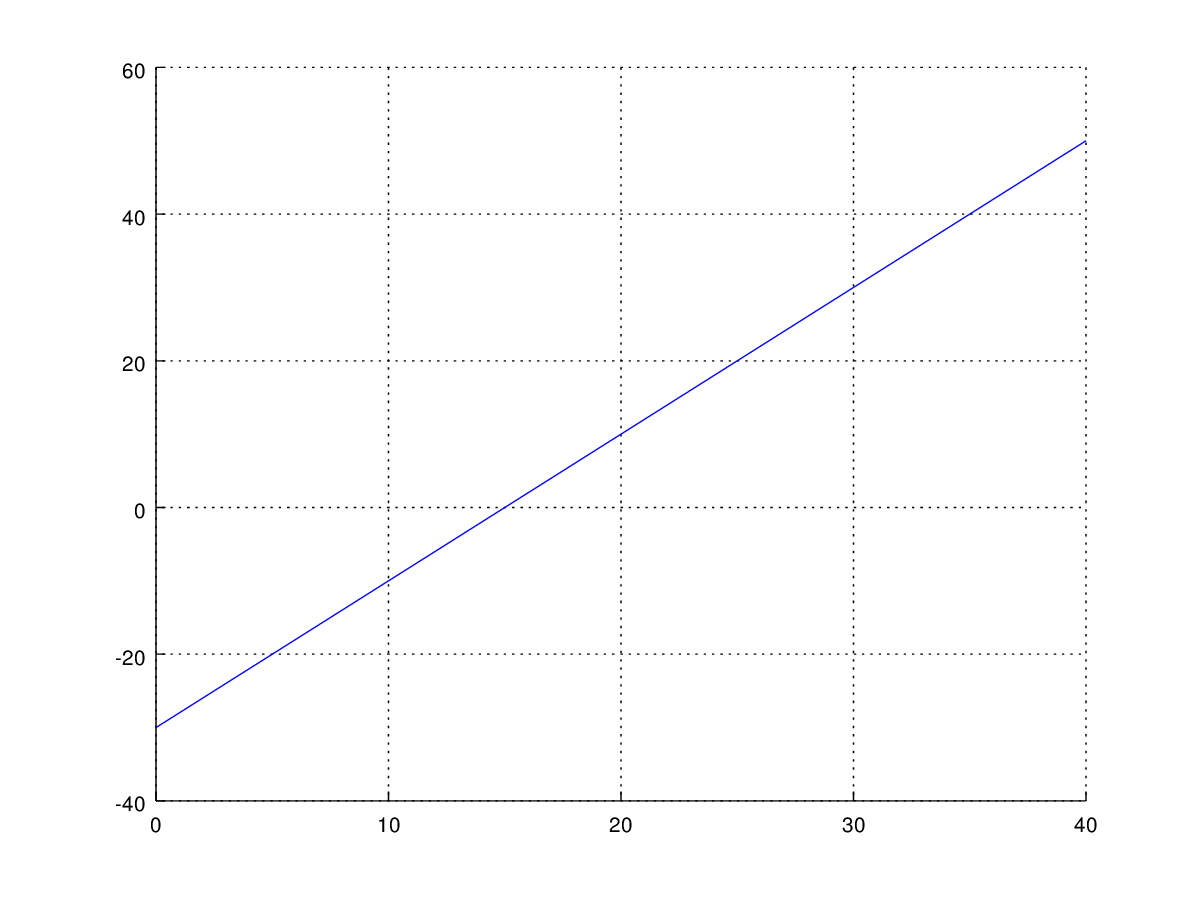
\includegraphics[width=0.5\textwidth]{imgs/ex1.png}
		\end{figure}
		\item Domínio: $\mathbb{N}$, contradomínio: $\mathbb{Z}$
		\item $f(x) \geq 0\implies 2x - 30 \geq 0 \implies x \geq 15$
	\end{enumerate}

	\item 
	\begin{enumerate}
		\item --
		\begin{figure}[H]
				\centering
				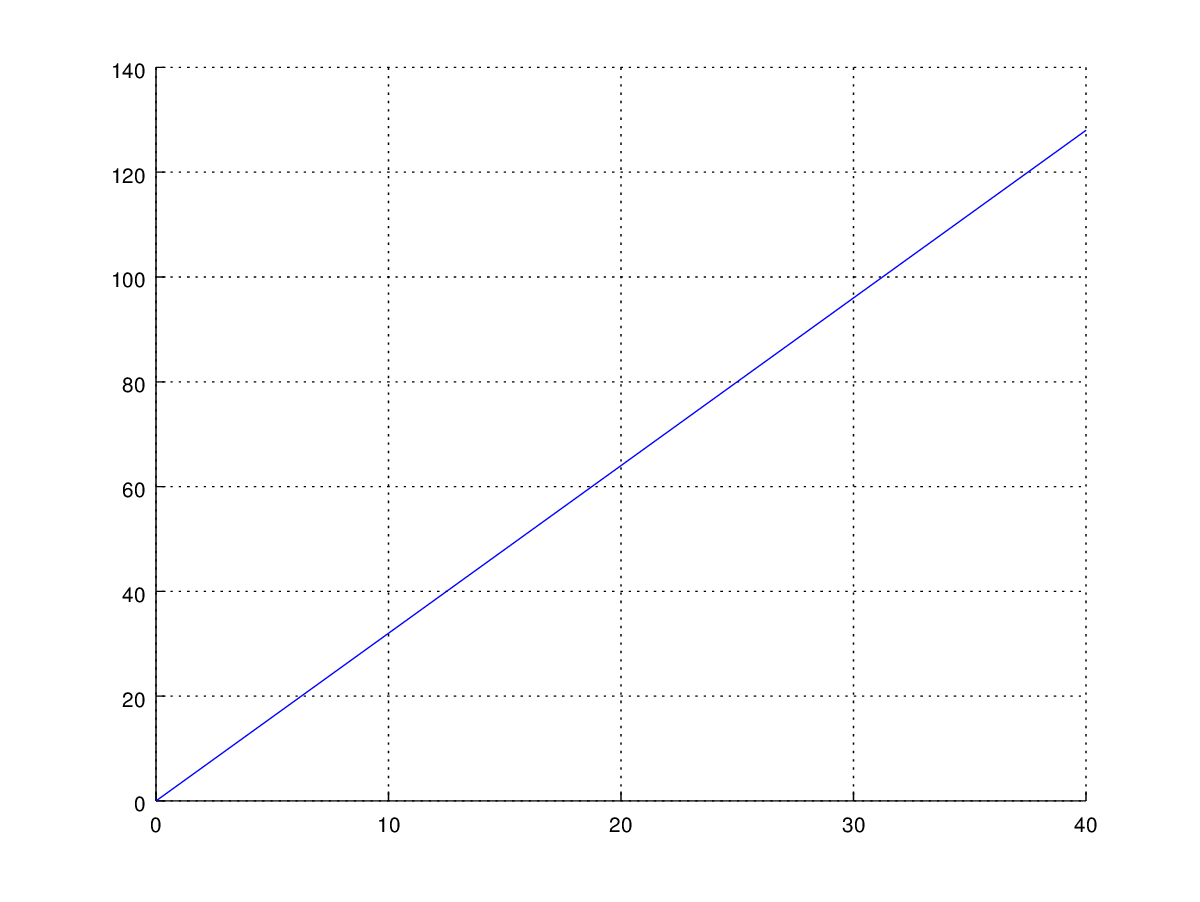
\includegraphics[width=0.5\textwidth]{imgs/ex2.png}
		\end{figure}
		\item Domínio: $\mathbb{R}$, contradomínio: $\mathbb{R}$
		\item $f(x) = 50 \implies 3.2x = 50 \implies x = \frac{50}{3.2} 
		      = 16.625$
	\end{enumerate}

	\item
	\begin{enumerate}
		\item Sim.
		\item Não pois há dois valores de saída para a mesma entrada.
		\item Sim.
	\end{enumerate}

	\item
	\begin{enumerate}
		\item Falso.
		\item Verdadeiro.
		\item Verdadeiro.
	\end{enumerate}

	\item 
	\begin{enumerate}
		\item $x = 0$
		\item $x = 25.938$
		\item $x = -\frac{1}{31.2} = -0.032$
	\end{enumerate}
\end{enumerate} 

\end{document}
